\documentclass[11pt,a4paper]{article}
\usepackage[left=25mm,top=4.0cm,right=25mm,bottom=4.0cm]{geometry}
\usepackage[utf8]{inputenc}
\usepackage{graphicx}

\newtheorem{1}{Definição}
\newtheorem{2}{Análise}
\newtheorem{3}{Observação}

\title {Projeto Álgebra Linear \\[1ex] \large Análise dos Componentes Principais em um Conjunto de Dados}

\author{Gabriel Luiz dos Santos Silva\\
João Pedro Borges Baeta
}

\date{06 dezembro 2022}

\begin{document}

\maketitle


%%%%%%%%%%%%%%%%%%%%%%%%%%%%%%%%%%%%%%%%%
% Introdução, Extração e Itens
%%%%%%%%%%%%%%%%%%%%%%%%%%%%%%%%%%%%%%%%%

\section{Introdução}
Este trabalho contém a análise de informações correspondentes ao custo de vida em quase 5000 cidades espalhadas pelo mundo. Toda a análise pode ser vista no JupyterNotebok chamado "principal-book-analysis.ipynb" no Github

\begin{description}
\item[Github:] https://github.com/gabrielluizone/Principal-Component-Analysis
\end{description}

Os dados foram extraídos da base de dados do site Numbeo (https://numbeo.com), onde se disponibiliza, por meio da contribuição dos mais de 700 mil contribuidores, o custo de vida de mais de 10 mil cidades espalhadas pelo planeta.  Os dados estão disponível para download no Kaggle pelo usuário mvieira101, chamado "global-cost-of-living"

\begin{3} \normalfont
Ao todo foram 54 itens utilizados para o cálculo do custo de vida nas cidades espalhadas pelo mundo. Para não haver a poluição da página, os itens podem ser visto na pasta "data" contendo o dicionário das colunas no Github
\end{3}

%%%%%%%%%%%%%%%%%%%%%%%%%%%%%%%%%%%%%%%%%
% Ferramentas
%%%%%%%%%%%%%%%%%%%%%%%%%%%%%%%%%%%%%%%%%
\section{Ferramentas e Metodologias Adotadas}
Foram utilizadas as seguintes ferramentas e bibliotecas para a análise, tratamento e calculos dos dados sobre o custo de vida das cidades no mundo.\\\\
• JupyterNotebook (Python)\\
• Pandas\\
• NumPy\\
• MatPlotLib\\
• Seaborn\\
• Sklearn\\

Para que seja possivel a realização do estudo, é necessário atender os requisitos para a realização da análise dos components principais, para isso, o conjunto de dados escolhido continha somente variváveis númericas com exceção dos países e suas cídades. Foram removidas linhas no qual, de acordo com o os próprios dados, eram considerados dados de baixa qualidade e os que continham dados nulos.

% Salvei sua lista no Keep para poupar página

%%%%%%%%%%%%%%%%%%%%%%%%%%%%%%%%%%%%%%%%%
% Análise 1
%%%%%%%%%%%%%%%%%%%%%%%%%%%%%%%%%%%%%%%%%
\section{Analisando os Componentes Principais}

\begin{2} \normalfont O primeiro passo do estudo, é nescessário criar a Matriz de Covariância, e para isso foi necessário padronizar as variáveis pela Matriz de Correlação, para  que sejam comparadas entre si. Para isso utiliza-se essa fórmula: (x- Média) / Desv. Padrão

% Fig 02
\begin{center}
    \includegraphics[width=12cm]{fig/02.png}
\end{center}

Após a utilização da fórmula acima, temos a matriz de correlação\\

% Fig 03
\begin{center}
    \includegraphics[width=14cm]{fig/03.png}
\end{center}

E pela utilização da variável "P", foi criada a matriz de Covariância\\

% Fig 04
\begin{center}
    \includegraphics[width=14cm]{fig/04.png}
\end{center}
\end{2}

%%%%%%%%%%%%%%%%%%%%%%%%%%%%
% Análise 2
%%%%%%%%%%%%%%%%%%%%%%%%%%%%
\begin{2} \normalfont Segundo passo, a partir da matriz de Covariância, precisamos encontrar os autovalores e os autovetores, e depois ordena-los em ordem decrescente

% Fig 05
\begin{center}
    \includegraphics[width=10cm]{fig/05.png}
    \includegraphics[width=16cm]{fig/06.png}
\end{center}
\end{2}

%%%%%%%%%%%%%%%%%%%%%%%%%%%%
% Análise 2
%%%%%%%%%%%%%%%%%%%%%%%%%%%%
\begin{2} \normalfont
Os autovalores estão representando a variabilidade dos dados, ou seja, quão acumulado a variância deles. A variância explicada de cada autovalor foi calcula pelo método abaixo:

\begin{center}
    \includegraphics[width=13cm]{fig/07.png}
    \includegraphics[width=10cm]{fig/08.png}
\end{center}

Como excolhemos cerca de 93\% da variância acumulada, usaremos 3 Componentes para assim, formamos a nossa nova matriz do conjunto de dados. Logo, deve-se realizar os calculos de a cordo com a formulas. Os calculos podem ser vistos no Github

$$T_r = XW_r$$
Onde $X$ é a nossa matriz (dataset) $n \times m$, $W_r$ é a matriz truncada em $r$ componentes e $T$ é a matriz com $r$ componentes principais.

\begin{center}
    \includegraphics[width=16.7cm]{fig/10.png}
\end{center}
\end{2}

\begin{2} \normalfont Após o processo, temos a seguinte matriz, contendo os três componentes, e colocamos os países como index para a visualização, entretanto, para facilitar a visualização dos componentes, selecionamos alguns países para não ficar muito extenso

\begin{center}
    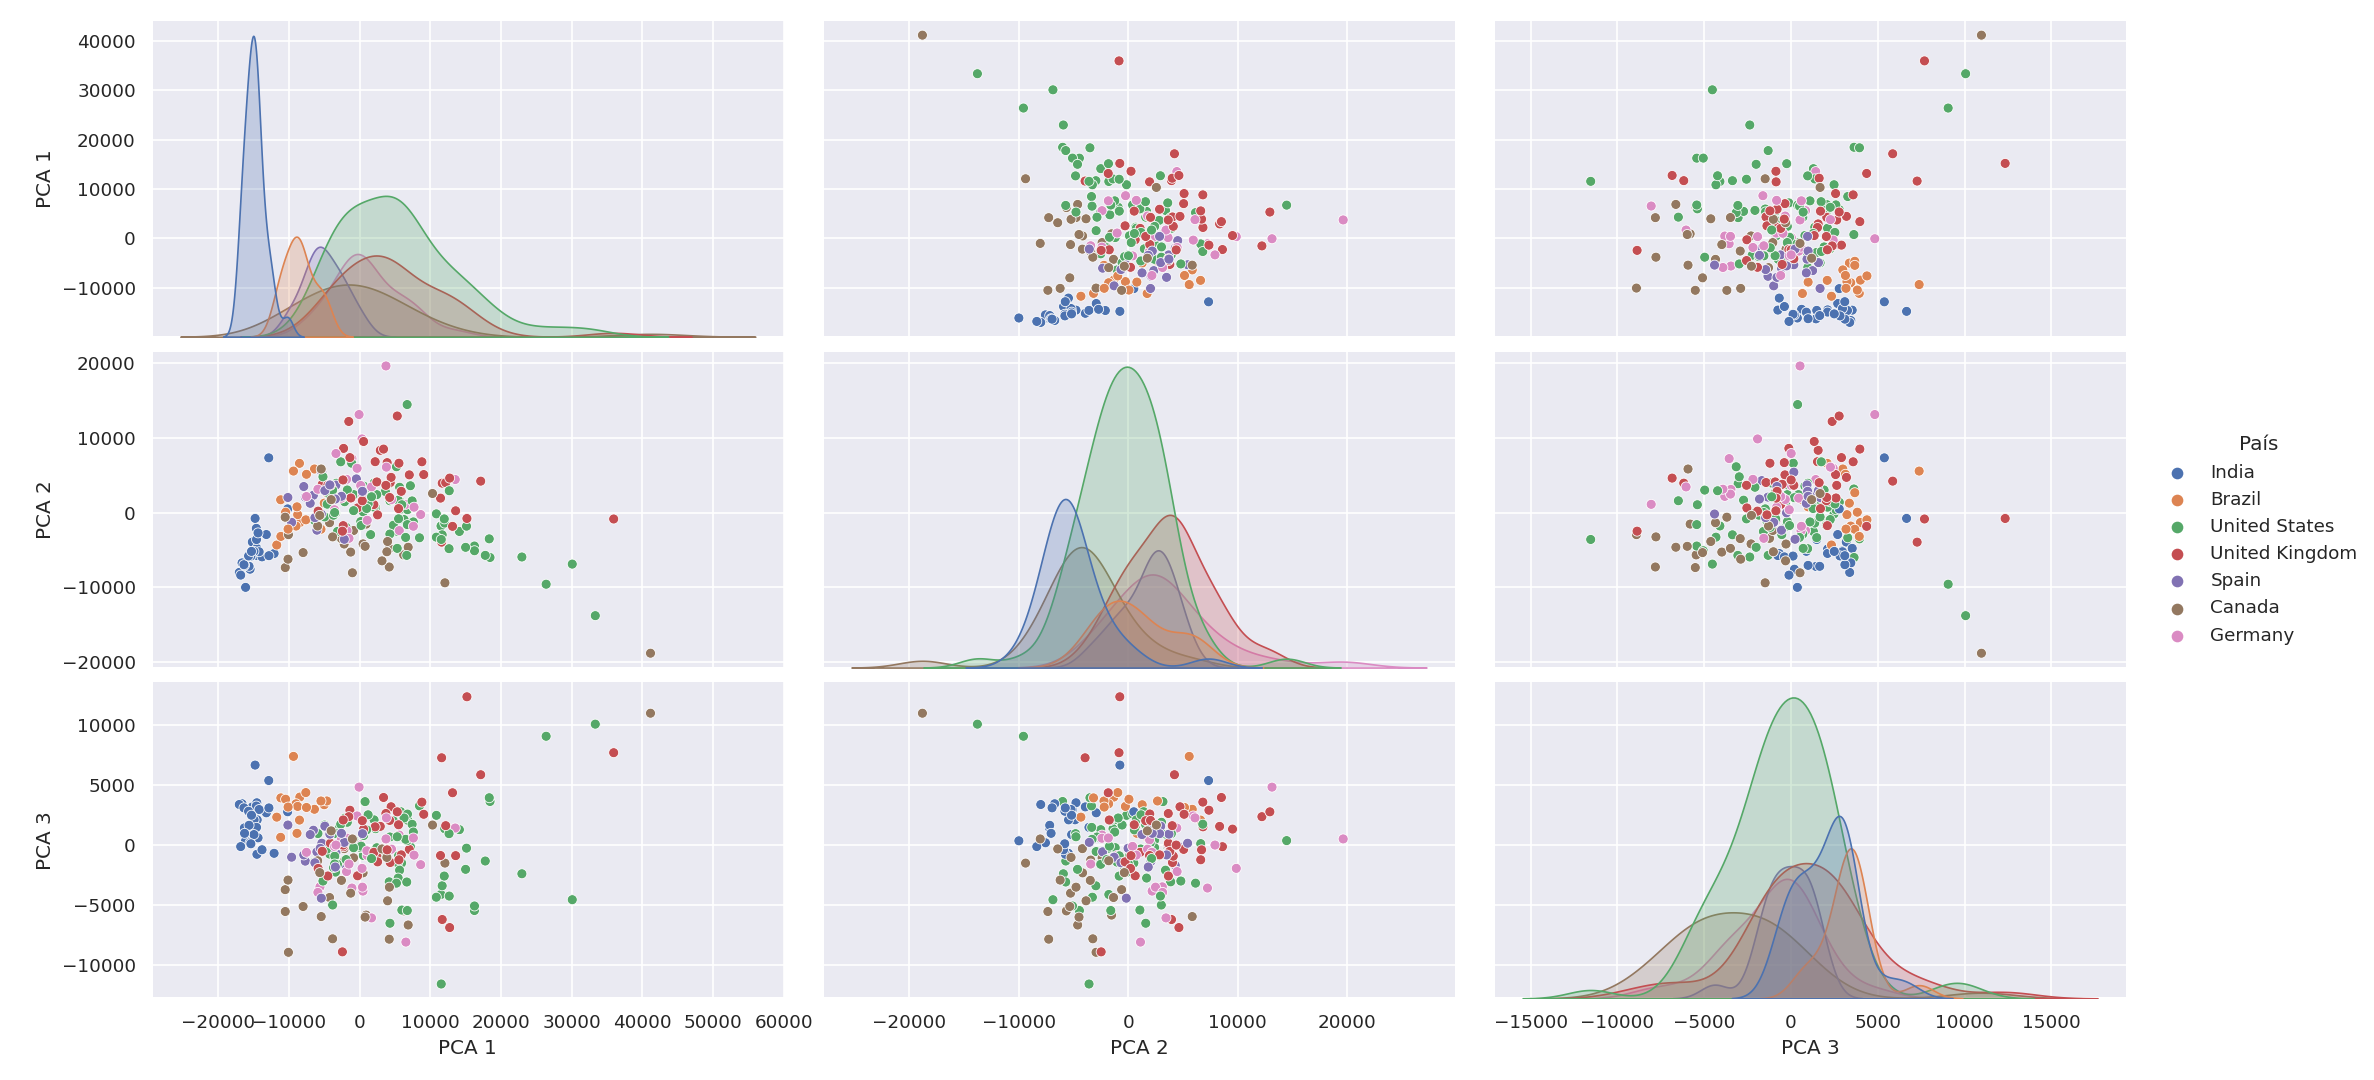
\includegraphics[width=17.2cm]{fig/plotplus.png}
\end{center}
\end{2}

\begin{2} \normalfont Visualização das direções dos Autovetores no 3º Plano

\begin{center}
    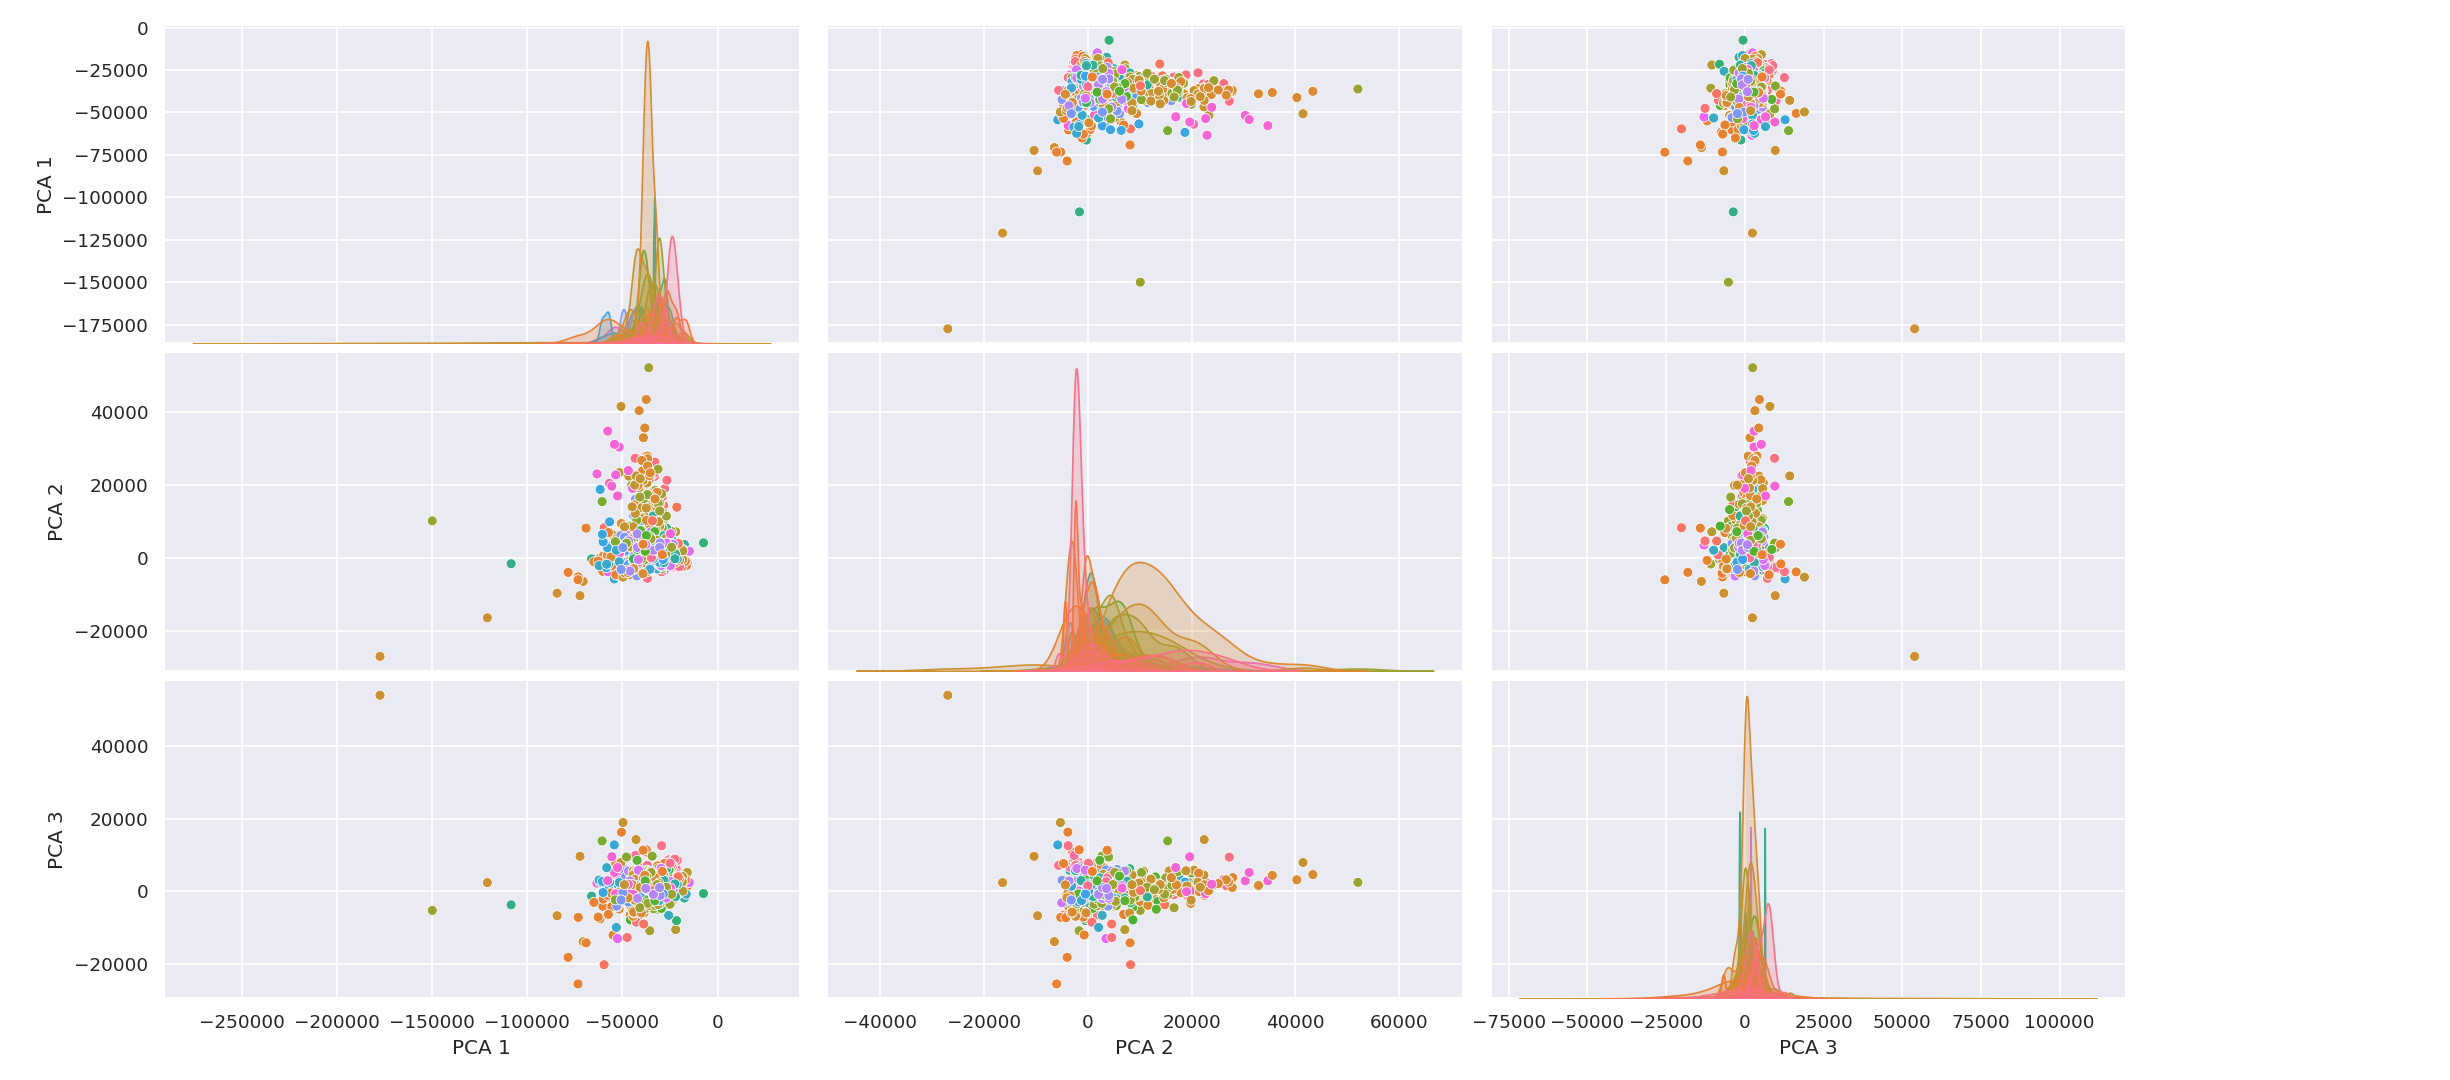
\includegraphics[width=10.8cm]{fig/plot02.png}
\end{center}
\end{2}

\end{document}
#
#⠀⠀⠀⠀⠀⠀⠀⠀⣀⣴⣶⣿⣿⣿⣿⣿⣿⣿⣶⣦⣀⠀⠀⠀⠀⠀⠀⠀
#⠀⠀⠀⠀⠀⠀⣤⣾⣿⣿⣿⣿⣿⣿⣿⣿⣿⣿⣿⣿⣿⣿⣄⠀⠀⠀⠀⠀
#⠀⠀⠀⠀⢀⣿⣿⣿⣿⣿⣿⣿⣿⣿⣿⣿⣿⣿⣿⣿⣿⣿⣿⣧⠀⠀⠀⢠
#⠀⠀⠀⠀⣿⣿⣿⣿⣿⣿⣿⣿⣿⣿⣿⣟⣛⣻⣿⣿⣟⣿⣿⣿⣷⠀⠀⠀
#⠀⠀⠀⠀⣿⣿⣿⣿⣿⣿⣿⣿⣿⣫⣽⣾⣻⣾⣿⣿⣿⣿⡿⣿⣿⠀⠀⠀
#⠀⠀⠀⢰⣿⣿⣻⣿⣿⣿⣿⣿⣿⣿⣿⣿⣿⠻⡿⠿⠟⠛⣟⣿⣽⠀⠀⠀
#⠀⠀⠀⠸⣿⣿⣿⣷⣿⣿⣿⣿⡿⠍⠈⠀⠁⣴⡆⠀⠀⠠⢭⣮⣿⡶⠀⠀
#⠀⡴⠲⣦⢽⣿⣿⣿⣿⣿⣟⣩⣨⣀⡄⣐⣾⣿⣿⣇⠠⣷⣶⣿⣿⡠⠁⠀
#⠀⠃⢀⡄⠀⢻⣿⣿⣿⣿⣽⢿⣿⣯⣾⣿⣿⣿⣿⣿⢿⣿⣿⡟⣿⠀⠀⠀
#⠀⠀⠣⠧⠀⢿⣿⣿⣿⣿⣿⣿⣿⣿⠟⢸⣿⠿⠿⠿⣧⠙⣿⣿⡿⠀⠀⠀
#⠀⠀⠀⠁⠼⣒⡿⣿⣿⣿⣿⣿⣿⣿⣠⣬⠀⠀⠀⠀⣾⣷⡈⣿⡇⠀⠀⠀
#⠀⠀⠀⠀⠀⠉⢳⣿⣿⣿⣿⣿⣿⣿⢟⠗⠼⠖⠒⠔⠉⠉⠻⣿⠇⠀⠀⠀
#⠀⠀⠀⠀⠀⠀⠈⣻⡿⣿⣿⣿⣿⡿⡀⣤⡄⠸⣰⣾⡒⣷⣴⣿⠀⠀⠀⠀
#⠀⠀⠀⠀⠀⠀⠂⢸⡗⡄⠘⠭⣭⣷⣿⣮⣠⣌⣫⣿⣷⣿⣿⠃⠀⠈⠀⠀
#⠀⠀⠀⠀⠀⠈⠀⢸⣿⣾⣷⣦⡿⣿⣿⣿⡿⢻⠞⣹⣿⣿⠏⠀⠀⠀⠀⠀
#⠀⠀⠀⠀⠀⢘⠀⠘⢻⡿⢿⣋⣤⣤⠌⠉⠛⠛⠀⠈⠉⠁⠀⠀⠀⠀⠀⡀      
#      